\documentclass[a0paper,landscape]{baposter}

\usepackage{lipsum}          % This is just for some blindtext

\usepackage{relsize}	       % For \smaller
\usepackage{url}			       % For \url
\usepackage{epstopdf}	       % Included EPS files automatically converted to PDF to include with pdflatex
\usepackage{multicol}        % Multi Columns

\usepackage{amsmath,amssymb} % math
\usepackage{natbib}
\usepackage{graphicx}

%%%%%%%%%%%%%%%%%%%%%%%%%%%%%%%%%%%%%%%%%%%%%%%%%%%%%%%%%%%%%%%%%%%%%%%%%%%%%%%%
%%% Utility functions %%%%%%%%%%%%%%%%%%%%%%%%%%%%%%%%%%%%%%%%%%%%%%%%%%%%%%%%%%
%%%%%%%%%%%%%%%%%%%%%%%%%%%%%%%%%%%%%%%%%%%%%%%%%%%%%%%%%%%%%%%%%%%%%%%%%%%%%%%%

%%% Save space in lists. Use this after the opening of the list %%%%%%%%%%%%%%%%
\renewcommand{\vec}[1]{\bm{#1}}
\newcommand{\vnabla}{\vec{\nabla}}

\renewcommand{\d}[1]{\text{d} #1}
\newcommand{\dxx}{\,\text{d}\vec{x}}
\newcommand{\dx}{\,\text{d}x}

\newcommand{\diff}[2]{\frac{\text{d}#1}{\text{d}#2}}
\newcommand{\idiff}[2]{\text{d}#1 / \text{d}#2}
\newcommand{\pdiff}[2]{\frac{\partial #1}{\partial #2}}
\newcommand{\pdifff}[2]{\frac{\partial^2 #1}{\partial #2^2}}
\newcommand{\ipdiff}[2]{\partial #1 / \partial #2}
\newcommand{\vdiff}[2]{\frac{\delta #1}{\delta #2}}
\newcommand{\ivdiff}[2]{\delta #1 / \delta #2}

%%%%%%%%%%%%%%%%%%%%%%%%%%%%%%%%%%%%%%%%%%%%%%%%%%%%%%%%%%%%%%%%%%%%%%%%%%%%%%%
%%% Document Start %%%%%%%%%%%%%%%%%%%%%%%%%%%%%%%%%%%%%%%%%%%%%%%%%%%%%%%%%%%%
%%%%%%%%%%%%%%%%%%%%%%%%%%%%%%%%%%%%%%%%%%%%%%%%%%%%%%%%%%%%%%%%%%%%%%%%%%%%%%%

\begin{document}
\typeout{Poster rendering started}

%%% General Poster Settings %%%%%%%%%%%%%%%%%%%%%%%%%%%%%%%%%%%%%%%%%%%%%%%%%%%
%%%%%% Eye Catcher, Title, Authors and University Images %%%%%%%%%%%%%%%%%%%%%%
\begin{poster}{
  columns=3,
	grid=false,
	borderColor=uniblue,
	headerColorOne=uniblue,
	headerColorTwo=uniblue,
	headerFontColor=white,
  headerheight=14em,
	boxColorOne=white,
  boxpadding=1em,
	headershape=rectangle,
	headerfont=\Large\textsf,
	textborder=none,
	background=shadetb,
  bgColorOne=white,
  bgColorTwo=white,
	headerborder=open,
  boxshade=plain,
  eyecatcher=false
}
%%% Eye Catcher %%%%%%%%%%%%%%%%%%%%%%%%%%%%%%%%%%%%%%%%%%%%%%%%%%%%%%%%%%%%%%%
{
}
%%% Title %%%%%%%%%%%%%%%%%%%%%%%%%%%%%%%%%%%%%%%%%%%%%%%%%%%%%%%%%%%%%%%%%%%%%
{\smaller This title is quite long as you can see}
%%% Authors %%%%%%%%%%%%%%%%%%%%%%%%%%%%%%%%%%%%%%%%%%%%%%%%%%%%%%%%%%%%%%%%%%%
{
  \vspace{1em}
  Max Mustermann\\
	{\smaller max.mustermann@stud-mail.uni-wuerzburg.de}
}
%%% Logo %%%%%%%%%%%%%%%%%%%%%%%%%%%%%%%%%%%%%%%%%%%%%%%%%%%%%%%%%%%%%%%%%%%%%%
{\begin{minipage}{20.0em}
    
\includegraphics[height=6em]{logo-uni}
  \end{minipage}
}

%%% Hintergrund %%%%%%%%%%%%%%%%%%%%%%%%%%%%%%%%%%%%%%%%%%%%%%%%%%%%%%%%%%%%%%%%%%
\headerbox{Hintergrund}{name=abstract,column=0,row=0}{
\begin{multicols}{2} 
  \lipsum[2-3]
\end{multicols}
}

%%% Box 1 %%%%%%%%%%%%%%%%%%%%%%%%%%%%%%%%%%%%%%%%%%%%%%%%%%%%%%%%%%%%%%%%%%%%%
\headerbox{Vorgehen}{name=box1,column=1,height=1}{
  % two columns, see: https://tex.stackexchange.com/questions/112983/beamer-columns-environment-in-article-document
  \begin{columns}
    \column{0.5\textwidth}
    \lipsum[1-1]
    \column{0.5\textwidth}
    \begin{itemize}
      \item one
      \item two
      \item three
      \item four
    \end{itemize}
  \end{columns}%

  \hhrule
  
  \lipsum[1]
    
}
\headerbox{Meine Grafik 1}{name=graph1,column=0,below=abstract,above=bottom}{
\begin{center}
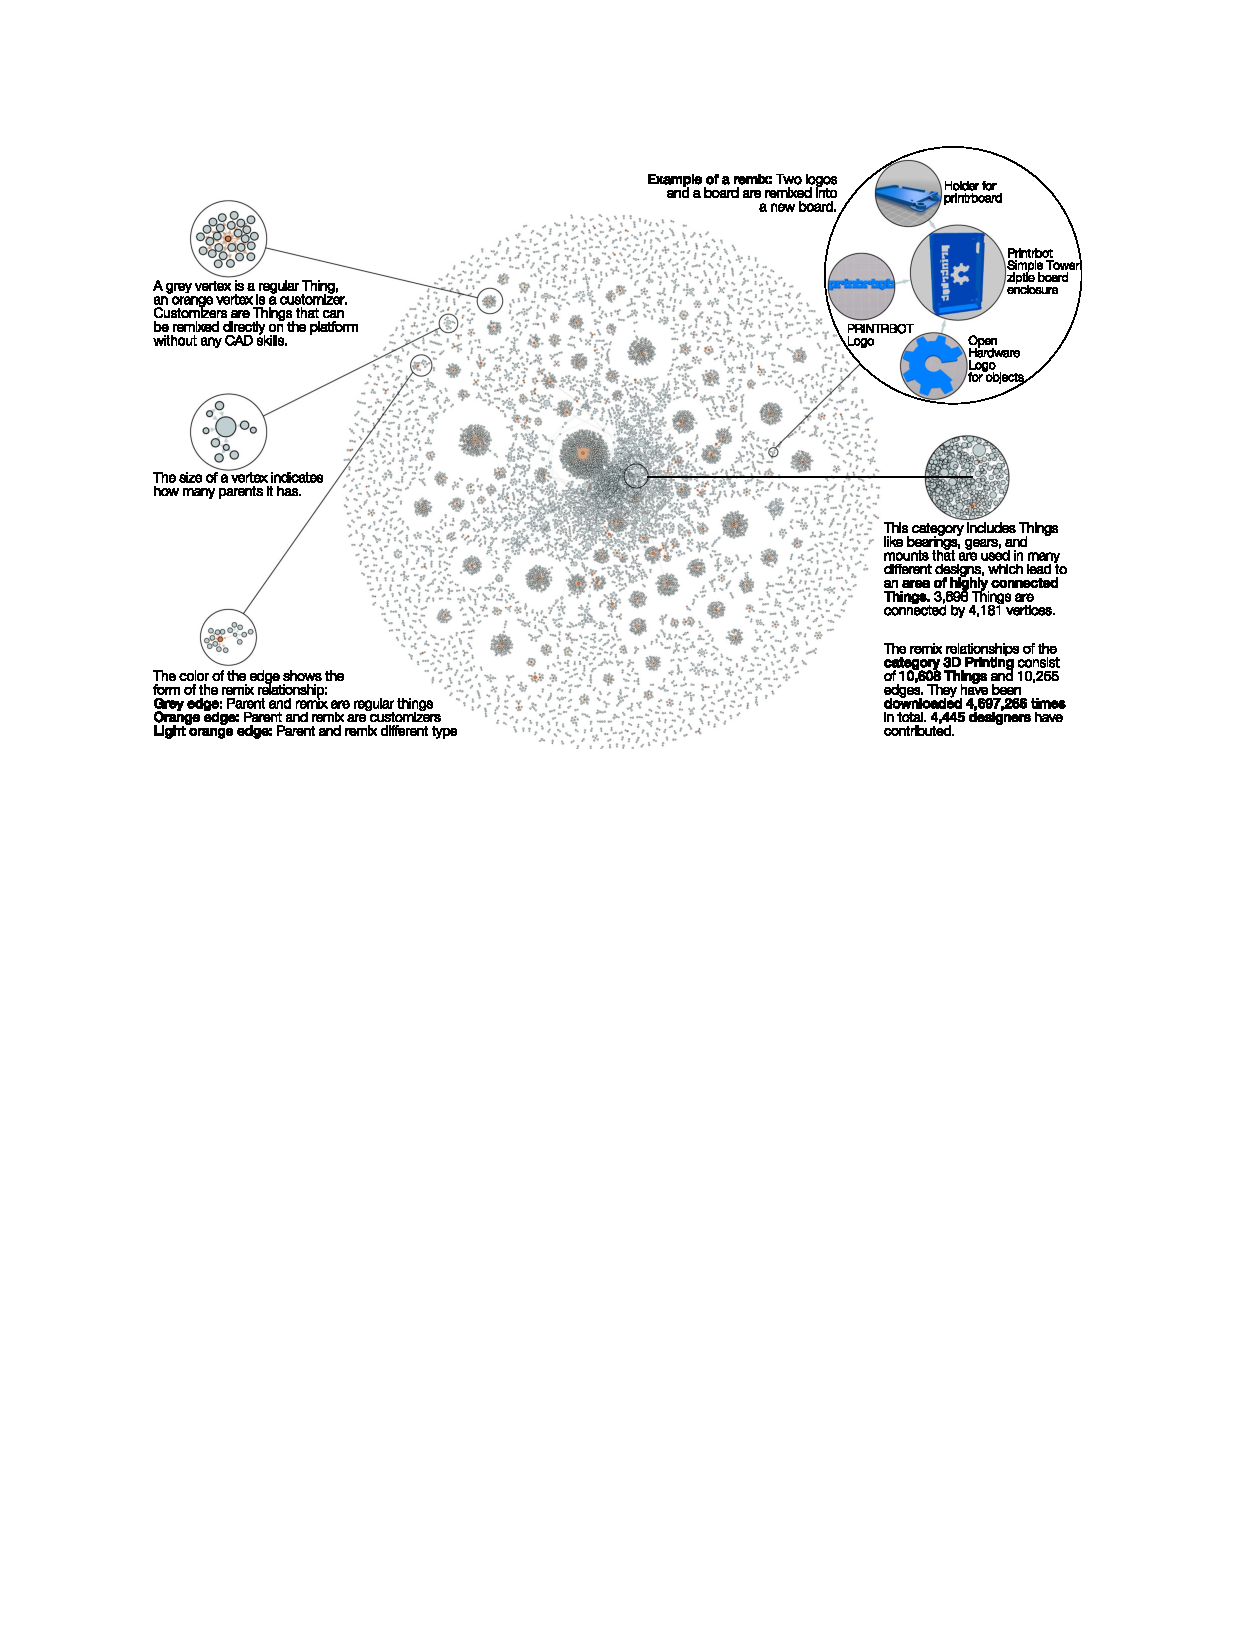
\includegraphics[width=0.9\textwidth]{ctc.pdf}    
\end{center}
}


%%% Box 2 %%%%%%%%%%%%%%%%%%%%%%%%%%%%%%%%%%%%%%%%%%%%%%%%%%%%%%%%%%%%%%%%%%%%%
\headerbox{Ergebnisse}{name=box2,column=2}{
  \begin{equation*}
    \int \vec{a} \cdot \vec{b} \dxx
  \end{equation*}

  \hhrule

    \lipsum[2-3]
    \citet{amor2004naive}
  
  \citet{optimization2014inc}
  
  \citet{hevner2010design}
}

%%% Box 3 %%%%%%%%%%%%%%%%%%%%%%%%%%%%%%%%%%%%%%%%%%%%%%%%%%%%%%%%%%%%%%%%%%%%%
\headerbox{Literatur}{name=box3,column=2,above=bottom,below=box2}{
\begingroup
\renewcommand{\section}[2]{}%
%\renewcommand{\chapter}[2]{}% for other classes
\bibliography{references}
\bibliographystyle{chicago}
\endgroup
}

\end{poster}
\end{document}
